\documentclass[border=4pt]{standalone}
\usepackage{tikz}
\usetikzlibrary{shapes.geometric,arrows.meta,positioning,calc}
\usepackage{amsmath}

\begin{document}
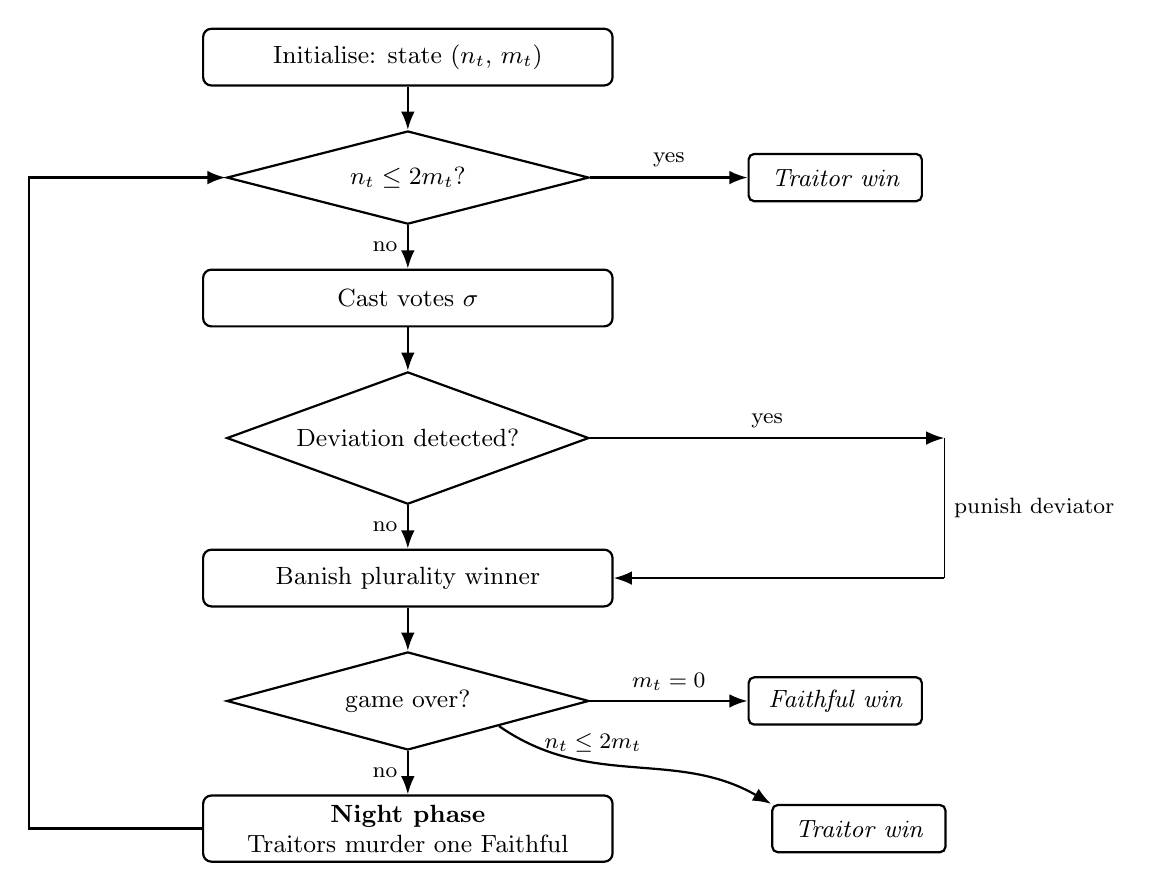
\begin{tikzpicture}[
  node distance=0.55cm,
  box/.style={
    rectangle, rounded corners=3pt, draw, thick,
    minimum width=5.2cm, minimum height=0.72cm,
    align=center, font=\small},
  dec/.style={
    diamond, draw, thick, aspect=2.5,
    minimum width=4.6cm, align=center, font=\small},
  res/.style={
    rectangle, draw, thick, rounded corners=2pt,
    minimum width=2.2cm, minimum height=0.60cm,
    align=center, font=\small\itshape},
  arr/.style={-Latex, thick},
]

  % ── Main spine ──────────────────────────────────────────────────────────
  \node[box]  (init)
      {Initialise: state \((n_t,\,m_t)\)};
  \node[dec,  below=0.55cm of init]    (wpre)
      {\(n_t \leq 2m_t\)?};
  \node[box,  below=0.55cm of wpre]    (votes)
      {Cast votes \(\sigma\)};
  \node[dec,  below=0.55cm of votes]   (detect)
      {Deviation detected?};
  \node[box,  below=0.55cm of detect]  (banish)
      {Banish plurality winner};
  \node[dec,  below=0.55cm of banish]  (wpost)
      {game over?};
  \node[box,  below=0.55cm of wpost]   (night)
      {\textbf{Night phase}\\
       Traitors murder one Faithful};

  % ── Terminal outcome nodes ───────────────────────────────────────────────
  \node[res, right=2.0cm of wpre]   (Tw1) {Traitor win};
  \node[res, right=2.0cm of wpost]  (Fw)  {Faithful win};
  \node[res, right=2.0cm of night]  (Tw2) {Traitor win};

  % ── Spine arrows ────────────────────────────────────────────────────────
  \draw[arr] (init)   -- (wpre);
  \draw[arr] (wpre)   -- node[left,  font=\footnotesize]{no}  (votes);
  \draw[arr] (votes)  -- (detect);
  \draw[arr] (detect) -- node[left,  font=\footnotesize]{no}  (banish);
  \draw[arr] (banish) -- (wpost);
  \draw[arr] (wpost)  -- node[left,  font=\footnotesize]{no}  (night);

  % ── Win condition exits ──────────────────────────────────────────────────
  \draw[arr] (wpre.east) --
      node[above, font=\footnotesize]{yes} (Tw1.west);
  \draw[arr] (wpost.east) --
      node[above, font=\footnotesize]{\(m_t = 0\)} (Fw.west);
  % Tw2 sits beside night, so the arrow curves well clear of the night box.
  \draw[arr] (wpost.south east) to[out=-35, in=150]
      node[above, font=\footnotesize, pos=0.35]{\(n_t \leq 2m_t\)}
      (Tw2.north west);

  % ── Deviation bypass: detect →yes→ right → down → into banish.east ──────
  % byp1: directly to the right of detect, past all right-side res nodes.
  % byp2: same x as byp1, at banish centre height.
  % The final segment goes leftward into banish.east (arrowhead there).
  \coordinate (byp1) at ($(detect.east) + (4.5cm, 0)$);
  \coordinate (byp2) at (byp1 |- banish);
  \draw[arr] (detect.east) --
      node[above, font=\footnotesize]{yes} (byp1);
  \draw      (byp1) --
      node[right, font=\footnotesize]{punish deviator} (byp2);
  \draw[arr] (byp2) -- (banish.east);

  % ── Loop back ───────────────────────────────────────────────────────────
  \draw[arr] (night.west) -- ++(-2.2, 0) |- (wpre.west);

\end{tikzpicture}
\end{document}
